\chapter{Differentiation}


\section{Wann und wozu verwendet man die finite Differenz?}

Die finite Differenz wird auf numerische Funktionen angewandt, die als Folge dargestellt werden und sich nur schwer analytisch differenzieren lassen. Sie wird verwendet, um die Ableitung von abgetasteten Daten zu finden, für die die erzeugende Funktion nicht bekannt ist.

\subsection{Vorwärtsdifferenz}

Die Vorwärtsdifferenz verwendet die Stichproben an einem Netzpunkt und den nächsten (vorwärts) gleichabständigen Analysepunkten, um die Ableitung am Netzpunkt zu berechnen. Die Fehlerschranke $O(h^2)$ beschreibt, dass der Fehler bzw. die Abweichung linear mit der Schrittweite anwächst. Das bedeutet: je kleiner $O(h^2)$, umso genauer ist 
\[ \frac{y_{k+1} - y_k}{h}\]
was die Annäherung der Ableitung beschreibt\textsc{\cite[S. 273]{Differentiationsformen}}.


\subsection{Rückwärtsdifferenz}

Die Rückwärtsdifferenz verwendet die Stichproben an einem Netzpunkt und den vorherigen (rückwärtigen) gleichmäßig beabstandeten Punkten, wie im Folgenden 

\[\frac{y_k - y_{k-1}}{h} \text{,}\]um die Ableitung zu berechnen\textsc{\cite[S. 273]{Differentiationsformen}}.

\subsection{Zentraldifferenz}
\label{sec:Zentraldifferenz}

Die Zentraldifferenz verwendet sowohl Vorwärts- als auch Rückwärts-Stichproben zur Berechnung der Ableitung am angegebenen Netzpunkt. Hier werden Taylorreihen höherer Ordnung genutzt, um mit $h < 1$ und 
\[
\frac{y_{k+1} - y_{k-1}}{2h}
\]
die Abweichung gering zu halten\textsc{\cite[S. 273]{Differentiationsformen}}.

Durch diese verschiedenen Annäherungen können Funktionen, die schwer analytisch abzuleiten sind, besser und genauer differenziert werden.

\section{Detaillierte Beschreibung und Genauigkeit}


\subsection{Erster Schritt zur numerischen Lösung}

Der erste Schritt zur numerischen Lösung erfordert die Diskretisierung des Lösungsgebiets. Dazu ist die Definition eines numerischen Gitters notwendig.


\subsection{Gitterstruktur bei Finite-Differenzen (FD) Diskretisierungsverfahren}

Das Gitter ist lokal strukturiert. Jeder Gitterknoten dient als Ursprung eines lokalen Koordinatensystems, wobei die Achsen des lokalen Koordinatensystems mit den Gitterlinien übereinstimmen.


\subsection{Eigenschaften und Anordnung der Gitterlinien}

Die Gitterlinien der gleichen Familie (z.B. $x = \text{const.}$ und $y = \text{const.}$) schneiden sich nicht. Gitterlinien unterschiedlicher Familien schneiden sich nur einmal. In drei Dimensionen schneiden sich drei Gitterlinien in jedem Knoten und bilden dort einen eindeutigen Schnittpunkt; diese Linien schneiden sich an keinem anderen Punkt.

\subsection{Genauigkeit}

Je geringer die Abstände der Gitterknoten sind, desto kleiner ist die entsprechende Abweichung der Annäherung der numerischen Lösung. Siehe in \ref{fig:Gitterknoten-Abstände}.

\begin{figure}[h]
    \centering
    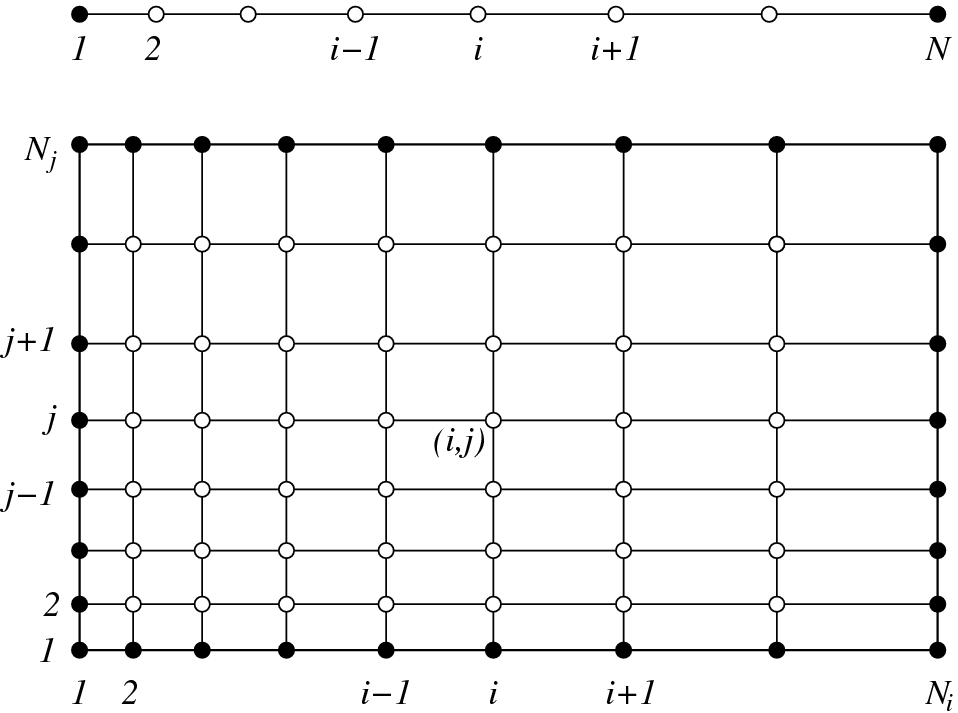
\includegraphics[scale=0.35]{images/Gitterknoten.png}
    \caption{Abstände der Gitterknoten}
    \label{fig:Gitterknoten-Abstände}
\end{figure}

\section{Praxisbeispiel FDM: Bezug zu Computer Engineering (CE)}

Dieses Praxisbeispiel zeigt die Anwendung der Finite-Differenzen-Methode (FDM) zur Berechnung der Wärmeleitung in dreidimensional geformten Blechkörpern\textsc{\cite{Praxisbeispiel_1}}.

\subsection{Herausforderungen bei der Simulation von Blechumformvorgängen}

Die Simulation von Blechumformvorgängen wird häufig mithilfe der Finite-Elemente-Methode (FEM) durchgeführt, wobei diese Simulationen meist isotherm erfolgen. Das bedeutet, dass dabei konstante Temperaturbedingungen angenommen werden. In der Praxis treten jedoch häufig gekoppelte thermisch-mechanische Effekte auf, die bei solchen isothermen Annahmen nicht berücksichtigt werden können. Dies führt zu numerischen Schwierigkeiten und ungenauen Ergebnissen.

\subsection{Vorteile der Finite-Differenzen-Methode (FDM)}

Im Gegensatz zur Finite-Elemente-Methode (FEM) wird die Finite-Differenzen-Methode (FDM) häufig zur Lösung von Wärmeleitungsproblemen eingesetzt. Dabei bietet die FDM mehrere Vorteile gegenüber der FEM:

Eine der Hauptstärken der FDM liegt in ihrer einfacheren Implementierung. Die Methode ist oft weniger komplex zu programmieren als die FEM, was sie besonders für Anwendungsbereiche attraktiv macht, in denen schnelle und unkomplizierte Lösungen gefragt sind.

Ein weiterer Vorteil der FDM ist ihre höhere Effektivität bei der Lösung von Wärmeleitungsproblemen. Die Methode kann in vielen Fällen effizienter und schneller zu Ergebnissen führen, was sie für bestimmte technische und physikalische Anwendungen besonders geeignet macht.


\subsection{Beschränkungen und Weiterentwicklungen der FDM}

Ein wesentlicher Nachteil der herkömmlichen FDM ist ihre Beschränkung auf einfache Geometrien, was ihre Anwendung auf komplexe Strukturen einschränkt. Um dieses Problem zu überwinden, wurde eine neue Variante der FDM entwickelt, die es ermöglicht, die Wärmeleitung in komplex geformten dreidimensionalen Blechen zu berechnen.

\subsection{Parametrisierung und Modellannahmen}

Die neue FDM nutzt eine geeignete Parametrisierung der Mittelfläche des Bleches, was eine effektive Lösung des Wärmeleitungsproblems erlaubt. Dabei wird die Annahme getroffen, dass die Bleche eine sehr geringe Dicke im Vergleich zu ihren anderen Abmessungen haben. Dies vereinfacht die mathematische Modellierung und reduziert den Rechenaufwand.

\subsection{Kopplung mit der Finite-Elemente-Methode (FEM)}

Ein bedeutender Vorteil der neuen FDM besteht darin, dass sie einfach mit der FEM gekoppelt werden kann. Diese Kopplung ermöglicht die simultane Simulation des Umformprozesses und der Wärmeleitung, was zu präziseren und realistischeren Ergebnissen führt. Durch die Kombination der Stärken beider Methoden können sowohl die mechanischen als auch die thermischen Effekte während des Umformprozesses berücksichtigt werden.

\subsection{Anwendungsbeispiele}

Diese neue Methode kann in verschiedenen industriellen Anwendungen eingesetzt werden, insbesondere in der Automobil- und Luftfahrtindustrie, wo die genaue Kontrolle der Temperatur während der Blechumformung entscheidend für die Qualität des Endprodukts ist. Die verbesserte Genauigkeit und Effizienz der neuen FDM tragen dazu bei, die Produktionsprozesse zu optimieren und die Materialeigenschaften gezielt zu beeinflussen.

\section{Implementation der FDM in Python}

\subsection{Vorgehen}
\label{sec:ImplFDM}

Zunächst soll das vorhin erwähnte Praxisbeispiel anhand eines Python-Programms mithilfe der \texttt{Numpy}- und \texttt{Matplotlib}-libraries implementiert werden, das die Finite-Differenzen-Methode (FDM) zur Berechnung der Wärmeleitung in einem dreidimensionalen Blechkörper verwendet. Der folgende Code zeigt die Implementierung der Methoden zur Berechnung der Deformation und der Temperaturverteilung, sowie die Visualisierung der Ergebnisse.

\subsection{Deformations- und Temperaturberechnung}

Die Berechnung der Deformation und der Temperaturverteilung erfolgt anhand der vorher beschriebenen Methoden. Dabei wird die Klasse \texttt{Derivative} (siehe \ref{lst:DerivativeClass}) aus dem Code-Abschnitt zur Approximation von Ableitungen verwendet, also die FDM.

\subsection{Python-Code für die \texttt{Derivative}-Klasse}
Nun wird die \texttt{Derivative}-Klasse näher betrachtet.

\subsubsection{Code der \texttt{Derivative}-Klasse}

Die  \texttt{Derivative}-Klasse bietet Methoden zur Berechnung der numerischen Ableitung einer Funktion mittels der Finite-Differenzen-Methode (FDM). Hier ist der vollständige Python-Code:

\begin{lstlisting}[language=Python, caption={Vollständiger Code der Derivative-Klasse}, label={lst:DerivativeClass}]
    import numpy as np
    from typing import Callable
    
    class Derivative:
        @staticmethod
        def of_order_1(
            f: Callable[[np.ndarray], np.ndarray],
            x: np.ndarray,
            h: float
        ) -> np.ndarray:
            assert h != 0
            return (f(x + h) - f(x - h)) / (2 * h)
    
        @staticmethod
        def of_order_2(
            f: Callable[[np.ndarray], np.ndarray],
            x: np.ndarray,
            h: float
        ) -> np.ndarray:
            assert h != 0
            return (f(x + h) - 2 * f(x) + f(x - h)) / (h * h)
\end{lstlisting}

\subsection{Erklärung der \texttt{Derivative}-Klasse und deren Methoden}

\paragraph{Klasse \texttt{Derivative}}

Die \texttt{Derivative}-Klasse bietet eine statische Methode zur numerischen Berechnung der ersten Ableitung einer Funktion. Sie verwendet die zentrale Differenzenmethode um die Ableitung an einer gegebenen Stelle zu approximieren.

\subsubsection{Methode \texttt{of\_order\_1}}

\paragraph{Parameter:}
\begin{itemize}
    \item \texttt{f}: Eine Funktion, von der die numerische Ableitung berechnet werden soll. Die Funktion sollte ein \texttt{np.ndarray} als Eingabe akzeptieren und ein \texttt{np.ndarray} als Ausgabe zurückgeben.
    \item \texttt{x}: Ein \texttt{np.ndarray}, das die Punkte enthält, an denen die Ableitung berechnet werden soll.
    \item \texttt{h}: Ein \texttt{float}, das die Schrittweite für die Finite-Differenzen-Methode angibt.
\end{itemize}

\paragraph{Rückgabewert:}
\begin{itemize}
    \item \texttt{np.ndarray}: Die numerisch berechnete erste Ableitung der Funktion an den angegebenen Punkten.
\end{itemize}

\paragraph{Funktionsweise:}
Die Methode \texttt{of\_order\_1} aus \ref{lst:DerivativeClass} berechnet die erste Ableitung einer Funktion \texttt{f} an den Punkten \texttt{x} mit einer Schrittweite \texttt{h}. Dies erfolgt durch die zentrale Differenzenmethode, welche in \ref{sec:Zentraldifferenz} numerisch dargestellt wird. Außerdem wird vorrausgesetzt, dass \texttt{h} nicht Null sein darf, da dadurch eine Nulldivision verhindert wird. Folglich wird die Formel

\[ f'(x) \approx \frac{f(x + h) - f(x - h)}{2h} \]

in diesem Kontext angewendet, da das $y$ an Index $k$ den Funktionswert an einer Stelle $x$ entspricht. Wird $k$ erhöht, nimmt die Funktion den Wert am nächsten Schritt an, also bei $x + h$. Dies gilt analog, für den Fall, wenn $k$ verkleinert wird.

Zusätzlich gibt es in \ref{lst:DerivativeClass} eine weitere statische Methode zur Berechnung der zweiten Ableitung einer Funktion. Diese Methode wird in der Implementierung des Kontexts nicht verwendet.

\subsubsection{Methode \texttt{of\_order\_2}}

\paragraph{Parameter:}
\begin{itemize}
    \item \texttt{f}: Eine Funktion, von der die numerische Ableitung berechnet werden soll. Die Funktion sollte ein \texttt{np.ndarray} als Eingabe akzeptieren und ein \texttt{np.ndarray} als Ausgabe zurückgeben.
    \item \texttt{x}: Ein \texttt{np.ndarray}, das die Punkte enthält, an denen die Ableitung berechnet werden soll.
    \item \texttt{h}: Ein \texttt{float}, das die Schrittweite für die Finite-Differenzen-Methode angibt.
\end{itemize}

\paragraph{Rückgabewert:}
\begin{itemize}
    \item \texttt{np.ndarray}: Die numerisch berechnete zweite Ableitung der Funktion an den angegebenen Punkten.
\end{itemize}

\paragraph{Funktionsweise:}
Die Methode \texttt{of\_order\_2} aus \ref{lst:DerivativeClass} berechnet die zweite Ableitung einer Funktion \texttt{f} an den Punkten \texttt{x} mit einer Schrittweite \texttt{h}. Dies erfolgt durch die zentrale Differenzenmethode der zweiten Ableitung, welche einen ähnlichen Aufbau wie die erste hat

\[f''(x) \approx \frac{f(x + h) - 2f(x) + f(x - h)}{h^2}\text{.}\]


\subsection{Python-Code für die Berechnung und Visualisierung}

\paragraph{Anwendungsbeispiel: Simulation der Blechverformung:}
Es wird angenommen, dass eine glatte Blechplatte im Zentrum verformt wird und die Temperaturverteilung über die Oberfläche simuliert werden soll. Der folgende Python-Code zeigt die Implementierung der Methoden zur Berechnung der Deformation und der Temperaturverteilung, sowie die Visualisierung der Ergebnisse. Es ist anzumerken, dass das Beispiel nur reale Maßnahmen annähert und nur als Darstellung für eine Mögliche Nutzung der FDM zur Berechnung der Steigung an den gewünschten Punkten.

\begin{lstlisting}[language=Python, caption={l1 und l2}, label={lst:linFunctions}]
    def l1(x: np.ndarray) -> np.ndarray:
        return 2.5 * x + 3.75


    def l2(x: np.ndarray) -> np.ndarray:
        return -2.5 * x + 3.75
\end{lstlisting}

\texttt{l1} und \texttt{l2} sind lineare Funktionen, die als Hilfe zur Modellierung des verformten Blechsstücks dienen. Betrachtet man den Querschnitt von \ref{fig:MetalSheetDeformation} auf der xz-Ebene bilden die Funktionen die zwei nicht parallelen Seiten eines Trapezes. 

\begin{lstlisting}[language=Python, caption={Deformationsfunktion}, label={lst:deformFunction}]
    def deformation_function(x: np.ndarray) -> np.ndarray:
        z = np.zeros_like(x)
        mask1 = (-1.5 < x) & (x < -1.3)
        mask2 = (-1.3 <= x) & (x <= 1.3)
        mask3 = (1.3 < x) & (x < 1.5)
    
        z[mask1] = l1(x[mask1])
        z[mask2] = 0.5
        z[mask3] = l2(x[mask3])
    
        return z
\end{lstlisting}

\texttt{deformation\_function} kombiniert die Funktionen aus \ref{lst:linFunctions} zur Modellierung der gesamten Verformung des Blechs. Es wird die \texttt{z}-Koordinate zurückgegeben.

\begin{lstlisting}[language=Python, caption={Temperaturfunktion}, label={lst:tempFunction}]
    def temperature_function(x: np.ndarray, z: np.ndarray) -> np.ndarray:
        h = 0.01
        gradient = np.abs(Derivative.of_order_1(deformation_function, x, h)) / 2.5
        temperature = gradient - z
        temperature[(-1.3 <= x) & (x <= 1.3)] = 0.4
        temperature = 1000 * temperature + 20
        return temperature
\end{lstlisting}

\texttt{temperature\_function} berechnet die Temperaturverteilung basierend auf der Verformung. Sie verwendet die Methode \texttt{of\_order\_1} der \texttt{Derivative}-Klasse (siehe \ref{lst:DerivativeClass}) zur Approximation der Ableitung. Die obere Fläche des Blechs bleibt konstant bei einer Temperatur, wärend die schiefen Flächen eine konstante Temperaturverteilung, die abhängig von der Höhe \texttt{z} sind, abbilden. Die Temperatur wird auf einen realistischen Bereich normalisiert.

\begin{lstlisting}[language=Python, caption={Plotten des Verformungsverfahren}, label={lst:PlotMetalDeformation}]
    def plot_simulation_metal_deformation():
        x = np.linspace(-5, 5, 500)
        y = np.linspace(-5, 5, 100)
        x, y = np.meshgrid(x, y)
    
        z = deformation_function(x)
    
        temperature = temperature_function(x, z)
    
        ls = LightSource(azdeg=315, altdeg=45)
        rgb = ls.shade(z, cmap=cm.jet, vert_exag=1, blend_mode='overlay')
    
        fig = plt.figure(figsize=(10, 6))
        ax = fig.add_subplot(111, projection='3d')
    
        surf = ax.plot_surface(
            x,
            y,
            z,
            rstride=1,
            cstride=1,
            facecolors=plt.cm.jet(temperature / 1000),
            linewidth=0,
            antialiased=True,
            shade=False
        )
    
        ax.set_xlabel('x')
        ax.set_ylabel('y')
        ax.set_zlabel('z')
    
        ax.set_zlim(0, 2)
    
        ax.set_title(...)
    
        plt.subplots_adjust(right=0.8)
    
        cbar_ax = fig.add_axes([0.85, 0.15, 0.03, 0.7])
        m = plt.cm.ScalarMappable(cmap=plt.cm.jet)
        m.set_array(temperature)
        fig.colorbar(m, cax=cbar_ax)
    
        ax.view_init(elev=30, azim=135)
    
        plt.show()
\end{lstlisting}
Die Funktion \texttt{plot\_simulation\_metal\_deformation} erstellt ein 3D-Oberflächendiagramm der Verformung mit der entsprechenden Temperaturverteilung. Die Abbildung \ref{fig:MetalSheetDeformation} zeigt den Plot dieser Funktion an. Es wird eine Farbskala verwendet, welche die Temperatur an den Stellen anzeigt, die benötigt wurde, um die Verformung durchzuführen. Das Temperaturintervall reicht von 20°C bis circa 900°C. Man erkennt  Beleuchtungseffekte werden verwendet, um die Visualisierung zu verbessern.

Schließlich wird die Methode \texttt{plot\_simulation\_metal\_deformation} aufgerufen:
\begin{lstlisting}
    plot_simulation_metal_deformation()
\end{lstlisting}

\begin{figure}[h]
    \centering
    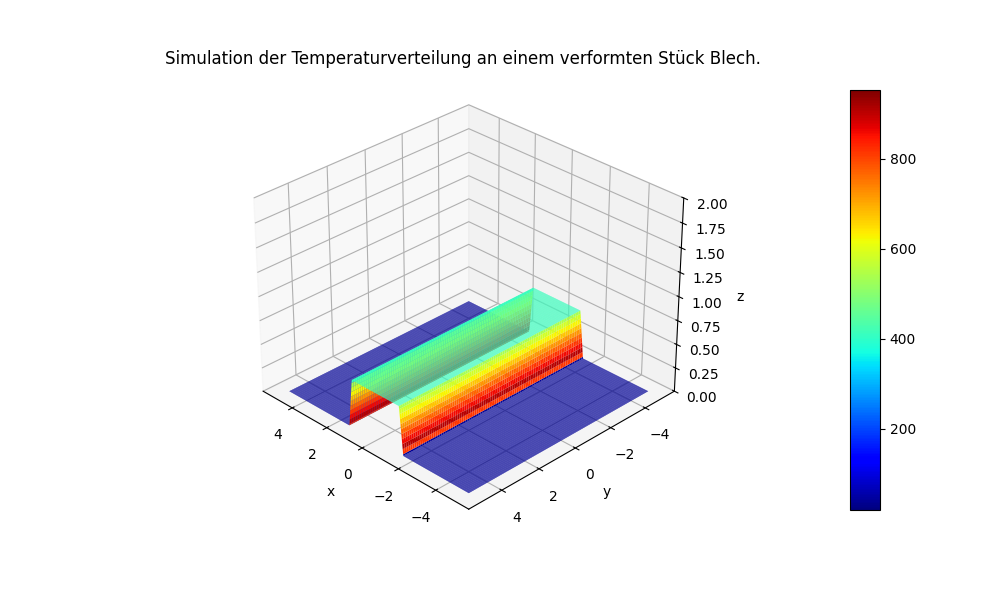
\includegraphics[width=\textwidth]{images/metal_sheet_deformation.png}
    \caption{Verformung und Temperaturverteilung einer Blechplatte}
    \label{fig:MetalSheetDeformation}
\end{figure}

\paragraph{Beobachtung: }
Die nicht verformten Stellen, für \texttt{x<=-1.5} und \texttt{x>=1.5} haben \texttt{z=0}, wurden daher nicht verändert und bleiben bei Raumtemperatur. Zwischen \texttt{-1.5<x<1.5} wird der beschriebene Verlauf deutlich, wie die Temperatur in Abhängigkeit der Steigung und der Höhe sich verändert. 

\subsection{Fazit}
Die Nutzung der FDM bei der Blechverformungen hilft, die Steigung für funktionale Verläufe bei der Verformung auszurechnen, um dafür den Temperaturaufwand zu berechnen. Die Umsetzung der Formel in Code ist simpel und führt zu nahen Approximationen für eine klein gewählte Schrittweite $h$.

Alternativ hätte man auch den plastischen Umformgrad analysieren und plotten können, für den auch die Steigung oder die Krümmung an bestimmten Punkten verwendet wird, wofür der Code aus \ref{lst:DerivativeClass} geeignet ist.